\chapter{Applied Methods}\label{chapter:applied-methods}

This chapter documents how the prototype micro-frontend architecture was built step by step. It starts with building the foundation of the application, continues with building the communication between the shell and remote application. Then, with the common caching layer and the reduction of queries, the basis for the evaluation of the hypothesis of the work was established. The final section is a comparison between the original and reduced queries.

\section{Implementation of a prototypical micro-frontend architecture}

The micro-frontend architecture that powers the prototype was developed using Webpack's Module Federation. The prototype contains a shell-application that loads all other micro-frontends. The architecture is divided into 9 widgets that display only simple data and 3 complex single-page applications.

The main part of the implementation is written in Angular. One micro-frontend was implemented with the frontend-framework React to show that the findings of this project are technology agnostic.

% TODO(FM): To detailed 
% I implemented one micro-frontend in React to show that the architecture is technology agnostic and if it can access the shared Apollo caching layer. For loading and rendering the React micro-frontend inside the host, I had to implement an adapter inside the shell-application. This adapter renders the React application inside a HTMLElement. It also provides the necessary configuration like the instance of the Apollo cache as context to the application. 

% Every micro-frontend is a complete Angular application that offers all of the features that Angular offers. 

A rough overview of the architecture is shown in figure \ref{figure:methods:ui-dashboard-architecture}. The icons inside the squares represent the technology used.

\ifshowImages
\begin{figure}[H]
\centering
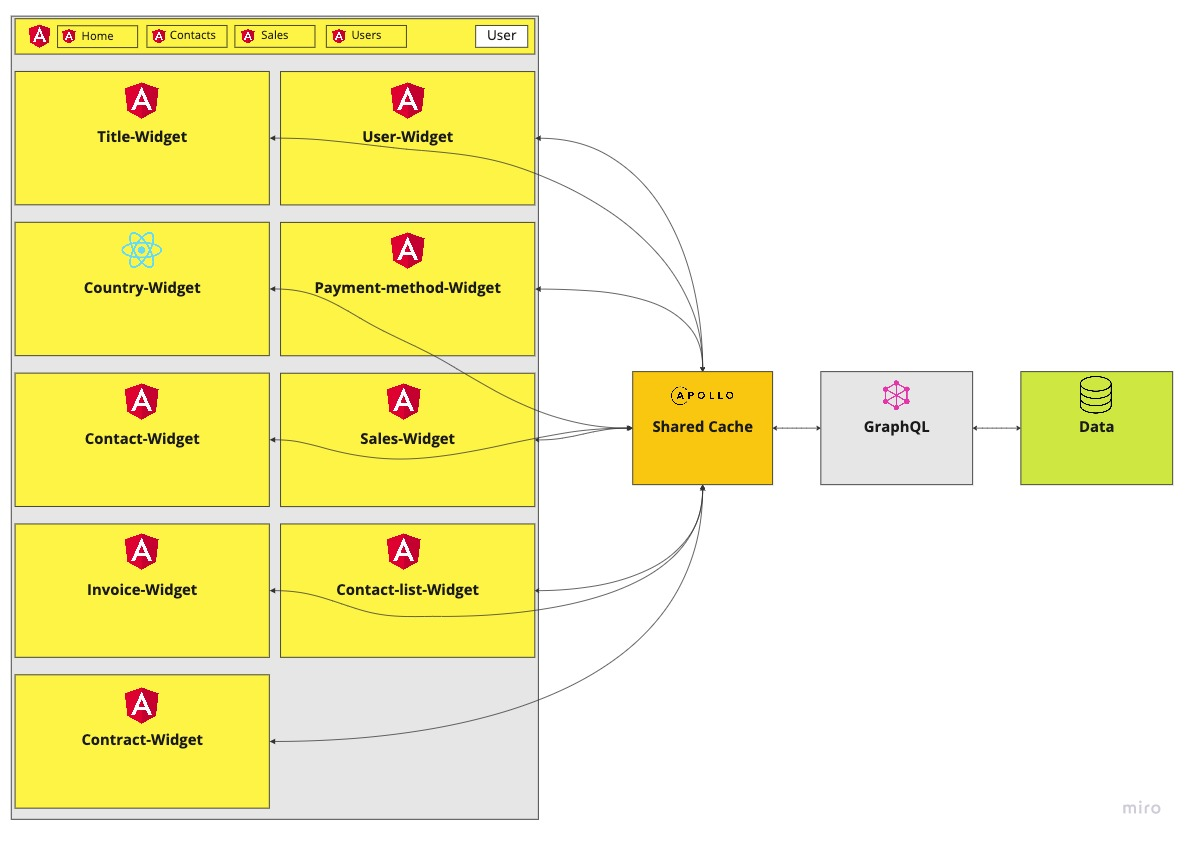
\includegraphics[width=0.8\linewidth]{images/ui-dashboard-architecture.jpg}
\caption{Architecture of the micro-frontend prototype.}\label{figure:methods:ui-dashboard-architecture}
\end{figure}
\fi

The functionality of the micro-frontends is encapsulated in modules that can be used by the shell application. Each icon of Angular and React represents such a module, as shown in figure \ref{figure:methods:ui-dashboard-architecture}. These modules can be used when the application is running in standalone mode, and the modules can be made accessible to the shell application via module federation.

\ifshowUnusedContent
% TODO(FM): Too detailed
% How a module can be exposed to be consumed by a remote application is shown in the listing \ref{code:methods:module-federation-config-expose}.

% \ifshowListings
% \begin{listing}[htbp]
% \begin{minted}{typescript}
% module.exports = {
%   name: 'contact',
%   exposes: {
%     './Module': 'apps/contact/src/app/remote-entry/entry.module.ts',
%   },
% };
% \end{minted}
% \caption{Module Federation config to expose an Angular module to be consumed.}\label{code:methods:module-federation-config-expose}
% \end{listing}
% \fi

% The host can configure its Module Federation to to be able to consume the entry.module.ts from the contact micro-frontend. The configuration can be seen in the listing \ref{code:methods:module-federation-config-consume}.

% \ifshowListings
% \begin{listing}[htbp]
% \begin{minted}{typescript}
% module.exports = {
%   name: 'host',
%   remotes: {
%     contact: 'contact@http://localhost:4202/remoteEntry.js'
%   },
% };
% \end{minted}
% \caption{Module Federation config that consumes an Angular module from a remote location.}\label{code:methods:module-federation-config-consume}
% \end{listing}
% \fi

% Inside the host application the remote module from the contact application can be easily referenced and routed to. The configuration of the route can be seen in listing \ref{code:methods:angular-route-to-remote-module}

% \ifshowListings
% \begin{listing}[htbp]
% \begin{minted}{typescript}
% const routes: Routes = [
%   {
%     path: 'contact',
%     loadChildren: () => 
%     loadRemoteModule(
%       'contact', 
%       './Module'
%     ).then((m) => m.UiContactRemoteEntryModule),
%   },
% }
% \end{minted}
% \caption{Route to the exposed remote-module from the contact application}\label{code:methods:angular-route-to-remote-module}
% \end{listing}
% \fi
\fi

\section{Communication from the shell- to the remote-application}\label{section:methods:communication-shell-remote}

To solve the problem of building a common caching layer, some form of communication between the shell and remote application had to be implemented. To ensure that the micro-frontends remain independent of each other, it should be avoided that they communicate directly with each other.

Angular provides a great tool for this use case, namely dependency injection. The shell application can provide services that can later be injected by the remote applications. This is very handy because the micro frontend can provide the same services as the shell application in standalone mode. Therefore, the remote module can be easily used within the remote and shell application.

\ifshowUnusedContent
% TODO(FM): Too detailed
% For example i implemented a layout-service that takes advantage of dependency injection. 

% \ifshowImages
% \begin{figure}[!htbp]
% \centering
% 
\includegraphics[width=1\linewidth]{images/prototype-screenshots/contact-header.png}
% \caption{Beispiel für die Beschriftung eines Buchrückens.}
% \end{figure}
% \fi

% \ifshowImages
% \begin{figure}[!htbp]
% \centering
% 
\includegraphics[width=1\linewidth]{images/prototype-screenshots/host-contact-header.png}
% \caption{Beispiel für die Beschriftung eines Buchrückens.}
% \end{figure}
% \fi
\fi

\section{Shared caching layer between the micro-frontends}

With the knowledge from the previous section \ref{section:methods:communication-shell-remote} a shared caching layer was implemented. Apollo GraphQL was chosen as GraphQL client for this prototype. It offers the most support for various frameworks and has a large community. The shell application can provide the instance of the GraphQL cache, which the micro-frontends can inject and use, when setting up their client, as seen in figure \ref{code:methods:graphql-client-cache-provider}. When running the micro-frontend in standalone mode, this provider has to be used inside the native application of the micro-frontend.

\ifshowUnusedContent
% TODO(FM): Too detailed
% For example the contact-application provides this object seen in listing \ref{code:methods:graphql-client-cache-provider} in its providers-array inside the core.module.ts. The host-application has the exactly same configuration inside its core.module.ts.
\fi

\ifshowListings
\begin{listing}[H]
\begin{minted}{typescript}
@NgModule({
  providers: [
    {
      provide: UI_GRAPHQL_CLIENT_CACHE,
      useValue: new InMemoryCache(),
    },
  ],
})
export class UiContactCoreModule {}
\end{minted}
\caption{Provide the instance of the cache to dependency injection.}\label{code:methods:graphql-client-cache-provider}
\end{listing}
\fi

\ifshowUnusedContent
% TODO(FM): Too detailed
% UI\_GRAPHQL\_CLIENT\_CACHE is an Angular Injection-token that can be used to provide injectable objects that can be used with dependency injection. (TODO: Injection token link)

% These provider must only be set inside the providers of the core.module.ts that the native application provides. Otherwise the remote-module would have their own instances of the GraphQL cache and the shared caching-layer would not work. 
\fi

Every micro-frontend can have their own instance of a GraphQL client. Only the GraphQL cache is shared between the different applications. Therefore, in theory, it is also possible that every micro-frontend consumes a different GraphQL API. 

\ifshowUnusedContent
% TODO(FM): Too detailed
% \ifshowListings
% \begin{listing}[htbp]
% \begin{minted}{typescript}
% @NgModule({
%   providers: [
%     {
%       provide: UI_GRAPHQL_CLIENT_OPTIONS_CONFIG,
%       useValue: {
%         shareCache: true,
%         persistCache: false,
%         useTypePolicies: true,
%         typePolicies: UI_CONTACT_APP_TYPE_POLICIES,
%       } as UiGraphQLClientOptionsConfig,
%     },
%   ],
% })
% export class UiContactRemoteCoreModule {}
% \end{minted}
% \caption{Extra configuration TODO}\label{code:methods:graphql-client-extra-configuration-options}
% \end{listing}
% \fi
\fi

To make it simple for the micro-frontends to use GraphQL, a function was written that creates the GraphQL client, seen in listing \ref{code:methods:graphql-client-creation}.

\ifshowListings
\begin{listing}[H]
\begin{minted}{typescript}
UiGraphQLClientOptionsModule.withConfig('contact-remote-app', { 
  provideGraphQLClientOptions: true,
}),
\end{minted}
\caption{Provide the instance of the cache as injectable.}\label{code:methods:graphql-client-creation}
\end{listing}
\fi

The first parameter of the function is a unique name for the GraphQL client instance. The unique name is mostly used for logging purposes. The second parameter is a configuration object whose options can be configured that no client is created.  

\ifshowUnusedContent
% For example the GraphQL client could be already provided inside the core-module of the shell-application and the remote-application injects that instance of the GraphQL client. These configuration options were largely added to test the shared caching layer with different options.
\fi

The final architecture follows the approach that each micro-frontend has a separate GraphQL client and a shared cache. This allows for the most flexibility as the GraphQL client can be configured individually by each micro frontend.


\ifshowUnusedContent
% My prototype creates 12 GraphQL clients, if every remote-application is loaded.

% \begin{enumerate}
%   \item host-native-app-graphql-client
%   \item contact-remote-app-graphql-client
%   \item sales-remote-app-graphql-client 
%   \item user-remote-app-graphql-client 
%   \item address-remote-widget-graphql-client
%   \item contact-list-remote-widget-graphql-client
%   \item contact-remote-widget-graphql-client 
%   \item contract-remote-widget-graphql-client
%   \item invoice-remote-widget-graphql-client 
%   \item person-remote-widget-graphql-client 
%   \item sales-remote-widget-graphql-client
%   \item user-remote-widget-graphql-client 
% \end{enumerate}
\fi

\section{Built a mechanism that reduces the size of queries}

Apart from sharing a cache instance, performance can be improved even further when using GraphQL in a shared architecture by removing fields from a query that are already in the cache.
However, the Apollo GraphQL client and no other GraphQL client with a caching layer provides this feature out of the box. Caching in Apollo works at the query level. So when a query is executed against the GraphQL backend, the results of the query are cached. If the same query is executed again, the cache is queried first to determine whether the query is already contained. If all queried fields of the new and old query are identical, the query results in a cache hit. However, if the new query queries fields that have not yet been queried by the old query and are therefore not yet in the cache, the query will result in a cache miss and fetched from the server. Consequently, identical queries that fetch different fields are always fetched from the server.

Consider the listing \ref{code:methods:query-all-users-reduction}. The left query fetches all users, and the right query fetches a user by id. Both queries fetch the same data, but two requests to the backend are made. The second query could completely be omitted, if the caching layer would be taken advantage of.

% For this case Apollo offers cache redirects, but the redirect works only if the list- and detail-view query the exact same fields. For example if the user micro-frontend query a list of users seen in listing \ref{code:methods:query-all-users-reduction} and when a user is selected, the detail-view might display the individual user like in listing \ref{code:methods:query-single-user}.

\ifshowListings
\begin{listing}[H]
\begin{minted}{typescript}
query {                                query User(id: ID!) {
  allUsers {                              User(id: id) {
    id                                      id
    username                                username
    email                                   email
    firstName                               firstname
    secondName                              secondName
  }                                       }    
}                                      }
\end{minted}
\caption{Query all users for the list-view.}\label{code:methods:query-all-users-reduction}
\end{listing}
\fi

\ifshowUnusedContent
% TODO(FM): too detailed
% In this case it is known that the user-data is already inside the cache, but fetched by a different query. The Apollo client doesn't know that and therefore tries to fetch the User from the server. But with Type-Policies we can tell the Apollo client where to look for the cached User. How to write such a redirect is shown in listing \ref{code:methods:user-cache-redirect}.

% \ifshowListings
% \begin{listing}[H]
% \begin{minted}{typescript}
% const client = new ApolloClient({
%   cache: new InMemoryCache({
%     typePolicies: {
%       Query: {
%         fields: {
%           User(_, { args, toReference }) {
%             return toReference({
%               __typename: 'User',
%               id: args.id,
%             });
%           }
%         }
%       }
%     }
%   })
% });
% \end{minted}
% \caption{Writing a cache-redirect for the User-type}\label{code:methods:user-cache-redirect}
% \end{listing}
% \fi

% That a detail-view and a list-view are identical is very rare in applications. Therefore this approach can't be used to reduce the size of network-requests effectively. And the approach is very verbose, because this redirect has to be written for every object type.
\fi

Many feature requests in the Apollo repository call for such a feature. While browsing GitHub, I found a project that provides drop-in replacements for Apollo's GraphQL query methods. And it provides the functionality to remove fields from a query that are already in the cache. However, the big problem was that the project was developed specifically for React and the dependencies were outdated. As a result, I couldn't install it and use it within the micro frontend written in React.

The next step was to rewrite the library in TypeScript and update the dependencies. While rewriting the library, some new features were added to still be able to exploit the cache-layer.

% But the library lacked the feature of cache-redirects. Therefore, the fields which were already queried by a list-view, couldn't be reduced when the detail-view was queries. I enhanced the implementation by adding a parameter, where a reference to an existing cache-object can be specified. If no reference is found in the cache, these reference to a cache-object is used to reduce the query.

In contrast to the original implementation, the new implementation is technology agnostic and can be used with every frontend framework that supports the Apollo client. For ease of use, I wrote adapters for React and Angular that have the same API as Apollo's original methods. The next section shows an example of the library in action.

\subsection{Example reduction}

This section contains an example of how query reduction works. The user navigates to the list view of all users, which executes the GraphQL query shown in listing \ref{code:methods:query-all-users}. After the query is fetched from the GraphQL backend, the fields in the query are cached

\ifshowListings
\begin{listing}[H]
\begin{minted}{typescript}
query allUsers {
  allUsers {
    id
    username
    email
    password
    firstName
    secondName
    gender
    Title {
      id
    }
    Salutation {
      id
    }
  }
}
\end{minted}
\caption{GraphQL query that queries all users.}\label{code:methods:query-all-users}
\end{listing}
\fi

The user then navigates to the detail view of a particular user. The left GraphQL query shown in the figure \ref{figure:code:comparison-user-reduced-user} is the original query that would normally be fetched from the backend. But with the help of reducing of the query with already existing data the right query is sent instead to the backend. Exactly the fields which were queried with the GraphQL query shown in listing \ref{code:methods:query-all-users} are removed. Therefore, 8 of the 16 fields were removed, reducing the size of the query by 50\%. In the next section, comparisons are made between the original queries and their reduced counterparts.

\ifshowImages
\begin{figure}[H]
\centering
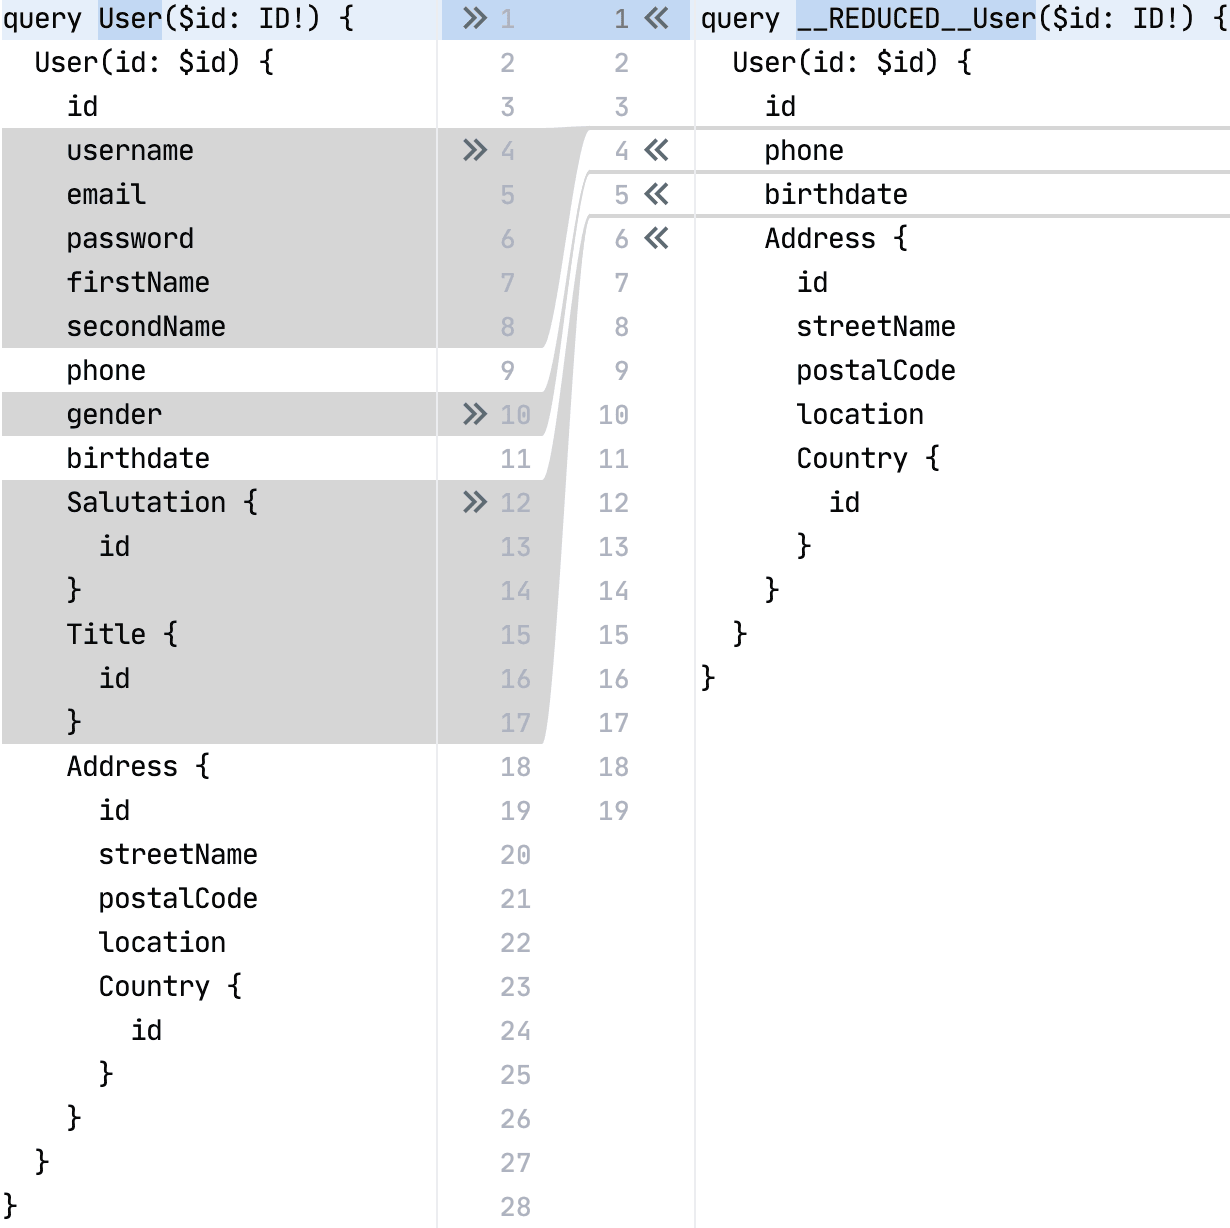
\includegraphics[width=0.6\linewidth]{images/reduction-graphql-examples/compare-user-reduced-user.png}
\caption{Comparison of the original user- and reduced user-query.}\label{figure:code:comparison-user-reduced-user}
\end{figure}
\fi

\subsection{Comparison between queries and reduced queries}

This section shows the difference in request- and response-size of different queries. The table \ref{table:code:comparison-user-reduction} shows the difference in size of the user-detail query, with the query reduction that was explained in the previous section. By removing 8 fields from the request, the size of the requests were reduced by 30\% or by 161 bytes. When querying 10 users a total of 1.61 KB can be saved. The response-size is reduced by 42\% on average. 2.55 KB in response-size is saved if 10 users are queried.

\ifshowTables
\begin{table}[H]
  \begin{tabular}{|l|l|l|l|l|}
  \hline
  Query & Request Diff (\%) & Request Diff (B) & Response Diff (\%) & Response Diff (B) \\
  \hline
  User & 30\% & 161 & 42\% & 257 \\
  \hline
  User & 30\% & 161 & 42\% & 257 \\
  \hline
  User & 30\% & 161 & 41\% & 257 \\
  \hline
  User & 30\% & 161 & 42\% & 244 \\
  \hline
  User & 30\% & 161 & 43\% & 251 \\
  \hline
  User & 30\% & 161 & 42\% & 271 \\
  \hline
  User & 30\% & 161 & 42\% & 249 \\
  \hline
  User & 30\% & 161 & 41\% & 263 \\
  \hline
  User & 30\% & 161 & 41\% & 248 \\
  \hline
  User & 30\% & 161 & 41\% & 252 \\
  \hline
  \hline
  \textbf{AVG} & \textbf{30\%} & - & \textbf{42\%} & -  \\
  \hline
  \textbf{SUM} & - & \textbf{1610 (1.61 KB)} & - & \textbf{2549 (2.55 KB)} \\
  \hline
  \multicolumn{5}{l}{16 fields, 8 Fields Removed, 8 remaining}
  \end{tabular}
  \caption{Comparison of the user-detail query in request- and response-sizes.}\label{table:code:comparison-user-reduction}
\end{table}
\fi

\ifshowUnusedContent
% TODO(FM): Too detailed
% The table \ref{table:code:comparison-contract-reduction} shows the difference for the contract-detail query. By running the list-query for all contracts 10 fields from the 17 can be removed from the query. Therefore only 7 from the 17 fields are remaining inside the query. The requests can be reduced by an average of 38\% or by 207 bytes. When using the application and querying 10 detail-views of the contract 2.07 KB can be saved. The size of the response from the GraphQL backend can be reduced by about 58\%. 3.96 KB in response-size is saved if 10 contracts are queried.

% \ifshowTables
% \begin{table}[ht]
%   \begin{tabular}{|l|l|l|l|l|}
%   \hline
%   Query  & Request Diff (\%)  & Request Diff (B) & Response Diff (\%) & Response Diff (B)  \\
%   \hline
%   Contract & 38\% & 207 & 58\% & 394 \\
%   \hline
%   Contract & 38\% & 207 & 58\% & 378 \\
%   \hline
%   Contract & 38\% & 207 & 59\% & 403 \\
%   \hline
%   Contract & 38\% & 207 & 60\% & 408 \\
%   \hline
%   Contract & 38\% & 207 & 60\% & 409 \\
%   \hline
%   Contract & 38\% & 207 & 57\% & 370 \\
%   \hline
%   Contract & 38\% & 207 & 58\% & 393 \\
%   \hline
%   Contract & 38\% & 207 & 58\% & 407 \\
%   \hline
%   Contract & 38\% & 207 & 59\% & 400 \\
%   \hline
%   Contract & 38\% & 207 & 58\% & 389 \\
%   \hline
%   \hline
%   \textbf{AVG} & \textbf{38\%} & - & \textbf{58\%} & - \\
%   \hline
%   \textbf{SUM} & - & \textbf{2070 (2.07 KB)} & - & \textbf{3951 (3.95 KB)} \\
%   \hline
%   \multicolumn{5}{l}{17 fields, 10 Fields Removed, 7 remaining}
%   \end{tabular}
%   \caption{Comparison of the contract-detail query in request- and response-sizes}\label{table:code:comparison-contract-reduction}
% \end{table}
% \fi

% \section{Persist the state of the cache}
% \section{Compared multiple GraphQL clients}
\fi
